\documentclass{article}

\usepackage{amsmath}
\usepackage{amsthm}
\usepackage{amssymb}
\usepackage{bbm}
\usepackage{fancyhdr}
% \usepackage{listings}
\usepackage{cite}
\usepackage{graphicx}
\usepackage{enumitem}
\usepackage{courier}
\usepackage{tikz}
\usepackage[pdftex,colorlinks=true, urlcolor = blue]{hyperref}

\usepackage{subfigure}

\oddsidemargin 0in \evensidemargin 0in
\topmargin -0.5in \headheight 0.25in \headsep 0.25in
\textwidth 6.5in \textheight 9in
\parskip 6pt \parindent 0in \footskip 20pt

% set the header up
\fancyhead{}
\fancyhead[L]{Stanford Aeronautics \& Astronautics}
\fancyhead[R]{Fall 2020}

%%%%%%%%%%%%%%%%%%%%%%%%%%
\renewcommand\headrulewidth{0.4pt}
\setlength\headheight{15pt}

\usepackage{xparse}
\NewDocumentCommand{\codeword}{v}{%
\texttt{\textcolor{blue}{#1}}%
}

\usepackage{xcolor}
\setlength{\parindent}{0in}

\title{AA 274A: Principles of Robot Autonomy I \\ Problem Set 3}
\author{Name: Parthiv Krishna      \\ SUID: 06330692}
\date{}

\begin{document}

\maketitle
\pagestyle{fancy} 

\section*{Problem 1: Camera Calibration}
\begin{enumerate}[label=(\roman*)]
\item Implemented \codeword{genCornerCoordinates} to to generate the world coordinates ($X$,$Y$) for each corner in each chessboard. Sample corner detection is below.

\includegraphics[width=0.9\textwidth]{Problem_1/chessboard_corners.PNG}

\item Implemented \codeword{estimateHomography} to estimate the homography matrix $H$ for each chessboard.
\item Implemented \codeword{getCameraIntrinsics} to estimate the linear intrinsic parameters of the camera.
\item Implemented \codeword{getExtrinsics} to estimate the rotation $R$ and translation $t$ of each chessboard when the images were captured.
\item Implemented \codeword{transformWorld2NormImageUndist} and \codeword{transformWorld2PixImageUndist} in order to switch from ($X$,$Y$,$Z$) to ($x$,$y$) or ($u$,$v$) in the undistorted image frames. 
\begin{enumerate}[label=(\alph*)] 
\item Sample output from \codeword{plotBoardPixImages} is on the next page.

\includegraphics[scale=0.8]{Problem_1/chessboard_pix.PNG}

\item Sample output from \codeword{plotBoardLocations} is below.

\includegraphics[width=0.9\textwidth]{Problem_1/chessboard_locations.PNG}

\end{enumerate}


\end{enumerate}

The calibration parameters are passed into \codeword{writeCalibrationYaml} to generate a configuration file.


\newpage

\section*{Problem 2: Line Extraction}
\begin{enumerate}[label=(\roman*)]
\item Implemented \codeword{SplitLinesRecursive}, \codeword{FindSplit}, \codeword{FitLine}, and \codeword{MergeColinearNeigbors} in \codeword{ExtractLines.py}.

\item Below are the extracted lines from the three datasets. The top left is \codeword{rangeData_5_5_180.csv}, the top right is \codeword{rangeData_4_9_360.csv}, and the bottom middle is \codeword{rangeData_7_2_90.csv}.
\begin{figure}[h]
    \subfigure{\includegraphics[width=.49\textwidth]{Problem_2/rangeData_5_5_180.png}}
    \hfill
    \subfigure{\includegraphics[width=.49\textwidth]{Problem_2/rangeData_4_9_360.png}}
\end{figure}
\begin{center}
    \includegraphics[width=.49\textwidth]{Problem_2/rangeData_7_2_90.png}
\end{center}

Below are the values for \codeword{MIN_SEG_LENGTH}, \codeword{LINE_POINT_DIST_THRESHOLD}, \\ \codeword{MIN_POINTS_PER_SEGMENT}, and \codeword{MAX_P2P_DIST} for the three different datasets.
\begin{center}
\begin{tabular}{ |c|c|c|c|c| } 
 \hline
  Dataset & Min Seg Len & Line Pt Dist Thresh & Min Pts Per Seg & Max P2P Dist \\ 
 5\_5\_180 & 0.05 & 0.02 & 2 & 0.5 \\ 
 4\_9\_360 & 0.05 &  0.01 & 2 & 1 \\
 7\_2\_90 & 0.05 & 0.15 & 3 & 1 \\
 \hline
\end{tabular}
\end{center}

\end{enumerate}

\newpage
\section*{Problem 3: Linear Filtering}
\begin{enumerate}[label=(\roman*)]
\item We zero pad $I$ to create $I'$.
$$I' = \begin{bmatrix}0 & 0 & 0 & 0 & 0 \\ 0 & 1 & 2 & 3 & 0 \\ 0 & 4 & 5 & 6 & 0 \\ 0 & 7 & 8 & 9 & 0 \\ 0 & 0 & 0 & 0 & 0 \end{bmatrix}$$
\begin{enumerate}[label=(\alph*)] 
\item $G = \begin{bmatrix}0 & 0 & 0 \\ 0 & 1 & 0 \\ 0 & 0 & 0 \end{bmatrix} \bigotimes I' = \begin{bmatrix}1 & 2 & 3 \\ 4 & 5 & 6 \\ 7 & 8 & 9 \end{bmatrix}$ \\ To find $G_{11}$ we can do $(0\cdot0) + (0\cdot0) + (0\cdot0) + (0\cdot0) + (1\cdot1) + (0\cdot2) + (0\cdot0) + (0\cdot4) + (0\cdot5) = 1$.
\item $G = \begin{bmatrix}0 & 0 & 0 \\ 0 & 0 & 1 \\ 0 & 0 & 0 \end{bmatrix} \bigotimes I' =\begin{bmatrix}2 & 3 & 0 \\ 5 & 6 & 0 \\  8 & 9 & 0 \end{bmatrix}$ \\ To find $G_{11}$ we can do $(0\cdot0) + (0\cdot0) + (0\cdot0) + (0\cdot0) + (0\cdot1) + (1\cdot2) + (0\cdot0) + (0\cdot4) + (0\cdot5) = 2$.
\item $G = \begin{bmatrix}-1 & 0 & 1 \\ -1 & 0 & 1 \\ -1 & 0 & 1 \end{bmatrix} \bigotimes I' = \begin{bmatrix}7 & 4 & -7 \\ 15 & 6 & -15 \\ 13 & 4 & -13 \end{bmatrix}$ \\ To find $G_{11}$ we can do $(-1\cdot0) + (0\cdot0) + (1\cdot0) + (-1\cdot0) + (0\cdot1) + (1\cdot2) + (-1\cdot0) + (0\cdot4) + (1\cdot5) = 7$. This mask is a derivative mask and calculates derivatives in the horizontal direction. Extreme values could be used to detect vertical edges, since going horizontally across a vertical edge would result in a quick change in color. This would show up as a large positive or negative image derivative. 
\item $G = \frac{1}{16} \begin{bmatrix}1 & 2 & 1 \\ 2 & 4 & 2 \\ 1 & 2 & 1 \end{bmatrix} \bigotimes I' = \begin{bmatrix}1.3125 & 2.25 & 2.0625 \\ 3.25 & 5 & 4.25 \\ 3.5625 & 5.25 & 4.3125 \end{bmatrix}$ \\ To find $G_{11}$ we can do $\frac{(1\cdot0) + (2\cdot0) + (1\cdot0) + (2\cdot0) + (4\cdot1) + (2\cdot2) + (1\cdot0) + (2\cdot4) + (1\cdot5)}{16} = \frac{21}{16} = 1.3125$. This mask performs a blur, and it would be useful in computer vision for reducing noise and/or variance, blurring prior to downscaling, and probably lots of other uses.
\end{enumerate}
\item As we saw when writing out the equations for the first pixel in each image manually, the value of the output $G(i,j)$ is the sum of the products of the corresponding entries in the filter $F$ and the padded image $I'$. In other words, $G(i,j) = \mathbf{f}^T\mathbf{t}_{ij}$ where $\mathbf{f}$ is a vector with all of the entries of $F$ (i.e., flattened/reshaped from a three-dimensional matrix to a one-dimensional vector) and $\mathbf{t}_{ij}$ is the "neighborhood" around $I_{ij}$, similarly flattened. A more explicit definition of the "neighborhood" around $I_{ij}$ is $I'_{i:i+k, j:j+l, :}$. In this way, the dot product can be represented as.
$$G(1,1)=\mathbf{f}^T\mathbf{t}_{1,1} = (F_{1,1,1}\cdot I'_{1,1,1}) + (F_{1,1,2}\cdot I'_{1,1,2}) + ... + (F_{1,1,c}\cdot I'_{1,1,c}) + (F_{1,2,1}\cdot I'_{1,2,1}) + ... + (F_{k,l,c}\cdot I'_{k,l,c})$$

This same idea holds if we try a different pixel, just $\mathbf{t}_{ij}$ would change as the neighborhood around the new pixel $I_{ij}$ is different. Thus, by constructing the vector $\mathbf{f}$ and the vector $\mathbf{t}_{ij}$ and then computing the dot product for each pixel, we can efficiently calculate the correlation output $G(i,j)$.

\newpage

\item Implemented the correlation operation within the \codeword{corr} function in \codeword{linear_filter.py}. Below are the output images. Top left is \codeword{corr_img_filt0.png}, top right is \codeword{corr_img_filt1.png}, bottom left is \codeword{corr_img_filt2.png}, and bottom right is \codeword{corr_img_filt3.png}.

\begin{figure}[h]
    \subfigure{\includegraphics[width=0.4\textwidth]{Problem_3/corr_img_filt0.png}}
    \hfill
    \subfigure{\includegraphics[width=0.4\textwidth]{Problem_3/corr_img_filt1.png}} \\
    \subfigure{\includegraphics[width=0.4\textwidth]{Problem_3/corr_img_filt2.png}}
    \hfill
    \subfigure{\includegraphics[width=0.4\textwidth]{Problem_3/corr_img_filt3.png}} \\
\end{figure}


\item The filters took 1-2 seconds each. One way that this process could be sped up is by calculating different pixels in parallel. Since any one output pixel depends only on the input image and the mask, there is no need to calculate each output pixel in any particular order which makes this a great candidate for parallelization. Additionally, if the filter can be decomposed into an outer product $F=\mathbf{ff}^T$ then it can be run as a correlation of $\mathbf{f}^T$ across the image and then a correlation of $\mathbf{f}$ across the image. This results in $O(2kmn)$ operations instead of $O(k^2mn)$; for large filters this can be quite significant! 

\item If every entry $F_{ij}$ is equal to $\sqrt{F_{ii}F_{jj}}$, then we can decompose $F$ into the outer product $F=\mathbf{ff}^T$. In other words, we must have that each entry in $F$ is equal to the square root of the product of the two entries on the main diagonal (top left to bottom right) of $F$ that are in its row and column. If this is true, $\mathbf{f}$ can be found by taking the square root of the entries of main diagonal (top left to bottom right) of $F$. In other words, $\mathbf{f}_i = \sqrt{F_{ii}}$.

\item Implemented \codeword{norm_cross_corr} in \codeword{linear_filter.py}.

\item In order to implement convolution with a correlation, we can simply flip the convolution filter $F$ horizontally and vertically to create $F'$. Computing correlation with the flipped filter $F'$ is equivalent to computing convolution with the original filter $F$.

\end{enumerate}

\newpage

\section*{Problem 4: Template Matching}
\begin{enumerate}[label=(\roman*)]
\item Implemented \codeword{template_match} in \codeword{template_matching.py}. The resulting detection of Valdo is below. 

\includegraphics[width=0.9\textwidth]{Problem_4/image_detections.png}
\item Ran template matching with the stop sign template \codeword{stop_signs/stop_template.jpg} on the other images available in the \codeword{stop_signs/} directory. Below are the outputs.

\begin{figure}[h]
    \subfigure{\includegraphics[height=0.11\textheight]{Problem_4/stop_signs/stop1_detection.png}}
    \hfill
    \subfigure{\includegraphics[height=0.11\textheight]{Problem_4/stop_signs/stop2_detection.png}}
    \hfill
    \subfigure{\includegraphics[height=0.11\textheight]{Problem_4/stop_signs/stop3_detection.png}}
    \hfill
    \subfigure{\includegraphics[height=0.11\textheight]{Problem_4/stop_signs/stop4_detection.png}}
    \hfill
    \subfigure{\includegraphics[height=0.11\textheight]{Problem_4/stop_signs/stop5_detection.png}}
    \\
\end{figure}

\item Template matching performs quite poorly on the other images. Some ways to improve template matching in addition to scaling would be template rotation, using additional templates, smoothing the image and the template to remove noise, or using different parts of the template to perform correlation.

\end{enumerate}

\newpage

\section*{Problem 5: Stop Sign Detection and FSM in ROS}
\begin{enumerate}[label=(\roman*)]
\item \codeword{supervisor.py} publishes message type \codeword{Pose2D} to \codeword{/cmd_pose}; this is the commanded goal pose for the robot. It also publishes message type \codeword{Twist} to \codeword{/cmd_vel}; this is used to command zero velocity when idle.


\item Copied \codeword{P2_pose_stabilization.py} from HW1 to \codeword{~/catkin_ws/src/asl_turtlebot/HW1} and modified \codeword{pose_controller.py} to subscribe to \codeword{/cmd_pose} and feed these poses to \\ \codeword{PoseController} to compute control commands.

\item Implemented the \codeword{camera_info_callback} function in \codeword{detector.py} to extract the focal lengths and principal points of the camera. 

\item Implemented \codeword{project_pixel_to_ray} in \codeword{detector.py} to com-pute the ray/direction (as a unit vector) of the stop sign in the camera’s frame of reference.

\item Below is the FSM diagram. close\_to($x_g$, $y_g$, $\theta_g$) returns true when the robot is at the target pose within some threshold. init\_stop\_sign() is called via a callback when a stop sign is detected within STOP\_MIN\_DIST, in this case, that's 0.5 meters. has\_stopped() returns true when it's been STOP\_TIME since the robot stopped, in this case, that's 3 seconds. has\_crossed() returns true when it's been CROSSING\_TIME since the robot started crossing the intersection, in this case, that's also 3 seconds. 

\begin{center}
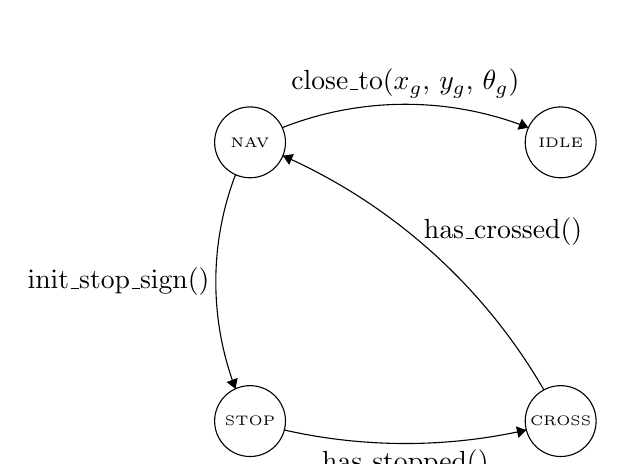
\begin{tikzpicture}[scale=0.15]
\tikzstyle{every node}+=[inner sep=0pt]
\draw [black] (18.6,-18.3) circle (3);
\draw (18.6,-18.3) node {\tiny{NAV}};
\draw [black] (44.9,-41.9) circle (3);
\draw (44.9,-41.9) node {\tiny{CROSS}};
\draw [black] (44.9,-18.3) circle (3);
\draw (44.9,-18.3) node {\tiny{IDLE}};
\draw [black] (18.6,-41.9) circle (3);
\draw (18.6,-41.9) node {\tiny{STOP}};
\draw [black] (21.328,-17.055) arc (111.50029:68.49971:28.436);
\fill [black] (42.17,-17.06) -- (41.61,-16.3) -- (41.24,-17.23);
\draw (31.75,-14.58) node [above] {close\_to($x_g$, $y_g$, $\theta_g$)};
\draw [black] (17.369,-39.166) arc (-159.13706:-200.86294:25.457);
\fill [black] (17.37,-39.17) -- (17.55,-38.24) -- (16.62,-38.6);
\draw (15.2,-30.1) node [left] {init\_stop\_sign()};
\draw [black] (41.997,-42.656) arc (-77.24805:-102.75195:46.425);
\fill [black] (42,-42.66) -- (41.11,-42.35) -- (41.33,-43.32);
\draw (31.75,-44.3) node [below] {has\_stopped()};
\draw [black] (21.379,-19.428) arc (66.12033:30.07397:47.984);
\fill [black] (21.38,-19.43) -- (21.91,-20.21) -- (22.31,-19.29);
\draw (40.02,-27.1) node [above] {has\_crossed()};
\end{tikzpicture}
\end{center}
\item Implemeted the FSM in \codeword{supervisor.py}.

\item Below is the path and velocity profile for the Turtlebot simulation. The velocity graph shows that the stop sign is reached around -0.6 minutes and the goal is reached around -0.2 minutes. Additionally, the logged output from \codeword{supervisor.py} shows the expected behavior: starting in nav mode, stopping for three seconds, crossing for three seconds, returning to nav mode, and then idling once the goal is reached.

\includegraphics[scale=0.42]{Problem_5_Plots.png} \includegraphics[scale=0.48]{Problem_5_Logs.png}

\end{enumerate}


\newpage
\section*{Extra Problem: Image Pyramids}
\begin{enumerate}[label=(\roman*)]

\item Implemented \codeword{half_downscale} in \codeword{image_pyramids.py}.

\item See (iv) for the result of calling \codeword{half_downscale} three times on \codeword{test_card.png}. The quality of this simple downscaling is pretty bad, with the central circle becoming very blocky and the thin alternating color lines on the outside edges becoming totally lost.

\item Blurring before downscaling will help because the blur modifies each pixel by adding some information about its neighbors. In this way, we avoid the blockiness from the previous method since we are using information from all of the pixels. Implemented \codeword{blur_half_downscale}.

\item Below is \codeword{test_card.png} (left), the result of calling \codeword{half_downscale} three times on \codeword{test_card.png} (middle), and the result of calling \codeword{blur_half_downscale} three times on \codeword{test_card.png} (right). Compared to \codeword{half_downscale}, \codeword{blur_half_downscale} certainly seems to retain more of the original "sense" of the image, in that the left and right edges are gray and the central circle seems more circular. Also, the vertical black/white bars in the lower half of the circle are more faithfully reproduced with the blur. That being said, it is still extremely blurry compared to the original, which is to be expected as there is less information in this image.


\begin{figure}[h]
    \subfigure{\includegraphics[width=0.33\textwidth]{Extra_Problem/test_card.png}}
    \hfill
    \subfigure{\includegraphics[width=0.33\textwidth]{Extra_Problem/out_simple_downscale.png}}
    \hfill
    \subfigure{\includegraphics[width=0.33\textwidth]{Extra_Problem/out_blur_downscale.png}}
    \\
\end{figure}

\item Implemented \codeword{two_upscale} within \codeword{image_pyramids.py}.

\item See (vii) for the result of calling \codeword{two_upscale} three times on \codeword{favicon-16x16.png}. This is very blocky and that is because each pixel in the original has become 64 pixels in the new image. Since there is no additional information or interpolation between each of the original pixels, the image is very blocky. 

\item Below is the result of calling \codeword{two_upscale} three times on \codeword{favicon-16x16.png} (left) and the result of calling \codeword{bilinterp_upscale} with scale=8 three times on \codeword{favicon-16x16.png} (right). The bilinear interpolation image is much less blocky and it's easier to make out the shape of the tree inside of the Stanford logo. This is because the interpolation has created additional information that makes it look less blocky and more blurry. 
\begin{figure}[h]
    \hspace{4cm}
    \subfigure{\includegraphics[width=0.3\textwidth]{Extra_Problem/out_simple_upscale.png}}
    \hfill
    \subfigure{\includegraphics[width=0.3\textwidth]{Extra_Problem/out_bilin_upscale.png}}
    \hspace{4cm}
\end{figure}

Intuitively, this works because the filter is a $(2s - 1)\times(2s - 1)$ square for scaling factor $s$. The central pixel has weight 1 and the other pixels decreasing in weight linearly as the distance from the center increases. Below is the filter for $s$=8, which is $15\times15$.

\includegraphics[scale=0.35]{Extra_Problem/filt_8.png}

So, if the filter is centered on a nonzero pixel in $I_{scaled}$, then the corresponding output in the result $G$ will be the same nonzero pixel. If the filter is centered on a zero pixel in $I_{scaled}$, the output in $G$ will be a weighted average of the nonzero pixels in $I_{scaled}$ that are within $s-1$ pixels of the center, weighted higher if they are closer to the center and lower if they're further from the center. This is the behavior we expect from bilinear interpolation. 

\item Implemented \codeword{template_match} in \codeword{scaled_template_matching.py}. Below is a sample detection image. 

\includegraphics[scale=0.45]{Extra_Problem/image_detections.png}

\item Ran template matching with Gaussian image pyramids with the stop sign template \\ \codeword{stop_signs/stop_template.jpg} on the other images available in the \codeword{stop_signs/} directory, the results are below. The performance is still extremely terrible with some images having a ton of false positives and others having no detections at all!

\begin{figure}[h]
    \subfigure{\includegraphics[height=0.11\textheight]{Extra_Problem/stop_signs/stop1_detection.png}}
    \hfill
    \subfigure{\includegraphics[height=0.11\textheight]{Extra_Problem/stop_signs/stop2_detection.png}}
    \hfill
    \subfigure{\includegraphics[height=0.11\textheight]{Extra_Problem/stop_signs/stop3_detection.png}}
    \hfill
    \subfigure{\includegraphics[height=0.11\textheight]{Extra_Problem/stop_signs/stop4_detection.png}}
    \hfill
    \subfigure{\includegraphics[height=0.11\textheight]{Extra_Problem/stop_signs/stop5_detection.png}}
    \\
\end{figure}

\end{enumerate}

\end{document}
